%% Determines the type of document (including standard settings for layout).
\documentclass[letterpaper]{article}



%% Package to control the size of a page: the standard margins used by LaTeX are
%% very wide!
\usepackage[margin=1in]{geometry}


%% Packages add functionality to the document. The AMS packages are standard
%% packages to support various mathematical notations. AMS stands for American
%% Mathematical Society, the organization that maintains these packages.
\usepackage{amsmath,amsthm,amssymb}

%% Theorems-like environments using functionality provided by amsthm.
\theoremstyle{plain}
\newtheorem{theorem}{Theorem}[section]
    %% [section] at the end specifies that theorems should be numbered
    %% per-section: Section x starts with theorem-like x.1 and so on, ...
\newtheorem{proposition}[theorem]{Proposition}
    %% [theorem] in the middle specifies: use the same counter as the theorem
    %% environment: here we number all theorem-like environments consecutively.
\newtheorem{corollary}[theorem]{Corollary}
\newtheorem{lemma}[theorem]{Lemma}
\theoremstyle{definition}
\newtheorem{definition}[theorem]{Definition}
\theoremstyle{remark}
\newtheorem{example}[theorem]{Example}
\newtheorem{remark}[theorem]{Remark}


%% Support for nicely formatted tables.
\usepackage{booktabs}


%% Support for colors & colors in tables.
\usepackage[table]{xcolor}

% Seven colors safe for use color blindness.
% Colors taken from doi:10.1038/nmeth.1618.
\definecolor{cbOrange}{RGB}{230,159,0}
\definecolor{cbSkyBlue}{RGB}{86,180,233}
\definecolor{cbBluishGreen}{RGB}{0,158,115}
\definecolor{cbYellow}{RGB}{240,228,66}
\definecolor{cbBlue}{RGB}{0,114,178}
\definecolor{cbVermillion}{RGB}{213,94,0}
\definecolor{cbReddischPurple}{RGB}{204,121,167}


%% Notation used in this document.
\newcommand{\n}{\mathbf{n}} %% Num. Replicas.
\newcommand{\f}{\mathbf{f}} %% Num. Faulty Replicas.

%% Misc. Math notation.
\newcommand{\BigO}{\mathcal{O}}
\newcommand{\abs}[1]{\lvert #1 \rvert}
\newcommand{\AName}[1]{\textsc{#1}}
\newcommand{\Var}[1]{\texttt{#1}}


%% Algorithms.
\usepackage{algorithm}
\usepackage[noend]{algorithmic}
\newcommand{\GETS}{:=}


%% Formatting SI-units.
\usepackage{siunitx}
\sisetup{per-mode=symbol}


%% TikZ: for creating figures.
\usepackage{tikz}

%% Configuration for figures: Nicer arrows.
\usetikzlibrary{arrows.meta}
\tikzset{>=Stealth}
\usetikzlibrary{automata,positioning,arrows}


%% pgfplots: drawing plots using TikZ.
\usepackage{pgfplots}
%% Configuration for plots: Use color-blind friendly colors.
\pgfplotscreateplotcyclelist{cbSafeList}{
    very thick,solid,cbOrange,every mark/.append style={solid},mark=*\\
    very thick,solid,cbSkyBlue,every mark/.append style={solid},mark=*\\
    very thick,solid,cbBluishGreen,every mark/.append style={solid},mark=*\\
    very thick,solid,cbYellow,every mark/.append style={solid},mark=*\\
    very thick,solid,cbBlue,every mark/.append style={solid},mark=*\\
    very thick,solid,cbVermillion,every mark/.append style={solid},mark=*\\
    very thick,solid,cbReddischPurple,every mark/.append style={solid},mark=*\\
    very thick,solid,black,every mark/.append style={solid},mark=*\\
}
\pgfplotsset{
    legend style={font=\small},
    compat=1.16,
    width=260pt,
    height=140pt,
    legend cell align=left,
    xlabel near ticks,
    ylabel near ticks,
    every axis/.append style={
        cycle list name=cbSafeList,
        ymin=0,
        enlargelimits=0.05,
        mark size=1pt,
        ylabel style={align=center},
        xlabel style={align=center},
        title style={align=center}
    }
}

%% PgfplotsTable: loading data files to use with pgfplots.
\usepackage{pgfplotstable}


%% Support for hyperlinks and urls. The setting ``colorlinks'' sets how links
%% are shown in the document (with a color, without underline). We put hyperref
%% last---it has a tendency to break other packages when loaded before them.
\usepackage[colorlinks]{hyperref}
\usepackage{graphicx}
\usepackage{pgffor}
\usepackage{caption}
\usepackage{tabularx}
\usepackage{enumitem}
\usepackage{fancyhdr}

\title{2AC3 Assignment 1}
\author{Luca Mawyin - 400531739}
\date{\today}
\renewcommand{\thesubsection}{\thesection.\alph{subsection}}

\begin{document}

\maketitle

\stepcounter{section}
\section*{\thesection.}

\begin{center}
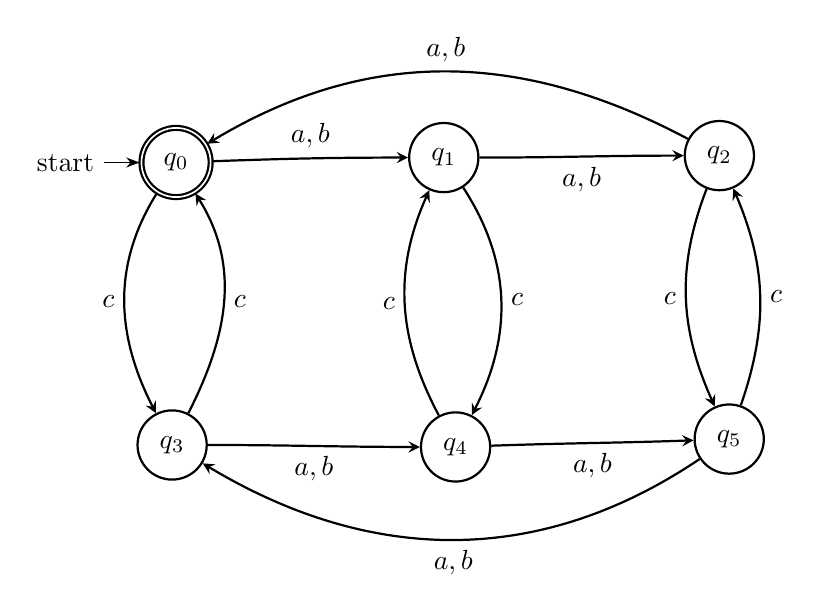
\begin{tikzpicture}[]
    \node[initial,thick,accepting,state] at (-2.55,2.625) (357edc8c) {$q_0$};
    \node[thick,state] at (0.85,2.6875) (ddeb69c0) {$q_{1}$};
    \node[thick,state] at (4.35,2.7125) (b0c4e59c) {$q_{2}$};
    \node[thick,state] at (-2.6,-0.9625) (1274030b) {$q_{3}$};
    \node[thick,state] at (1,-0.9875) (93bcf703) {$q_{4}$};
    \node[thick,state] at (4.475,-0.8875) (36c43620) {$q_{5}$};
    \path[->, thick, >=stealth]
    (357edc8c) edge [above,in = 180, out = 2] node {$a,b$} (ddeb69c0)
    (357edc8c) edge [left,in = 117, out = -122] node {$c$} (1274030b)
    (ddeb69c0) edge [below,in = -180, out = 0] node {$a,b$} (b0c4e59c)
    (ddeb69c0) edge [right,in = 63, out = -57] node {$c$} (93bcf703)
    (b0c4e59c) edge [left,in = 114, out = -111] node {$c$} (36c43620)
    (b0c4e59c) edge [above,in = 31, out = 152] node {$a,b$} (357edc8c)
    (1274030b) edge [below,in = 180, out = 0] node {$a,b$} (93bcf703)
    (1274030b) edge [right,in = -58, out = 63] node {$c$} (357edc8c)
    (93bcf703) edge [below,in = -178, out = 2] node {$a,b$} (36c43620)
    (93bcf703) edge [left,in = -114, out = 118] node {$c$} (ddeb69c0)
    (36c43620) edge [below,in = -31, out = -146] node {$a,b$} (1274030b)
    (36c43620) edge [right,in = -67, out = 71] node {$c$} (b0c4e59c)
    ;
\end{tikzpicture}
\end{center}

$q_0$ acts as both the initial state and the final state. This allows $\epsilon$ to hold trivially. Furthermore, there are two rows of states that act similarly. The first row of states ($q_0,q_1,q_2$) represents an even number of $c$. The second row of states ($q_3,q_4,q_5$) represents an odd number of $c$. Both rows of states connect by cycling through $a$ and $b$ until the sum is divisible by 3. If the number of $c$ is odd, the only way to get to the final state is to increase the number of $c$ by one, causing there to be an even amount. DFA accounts for everywhere that the $c$ may be placed.

\stepcounter{section}
\section*{\thesection.}

\begin{center}
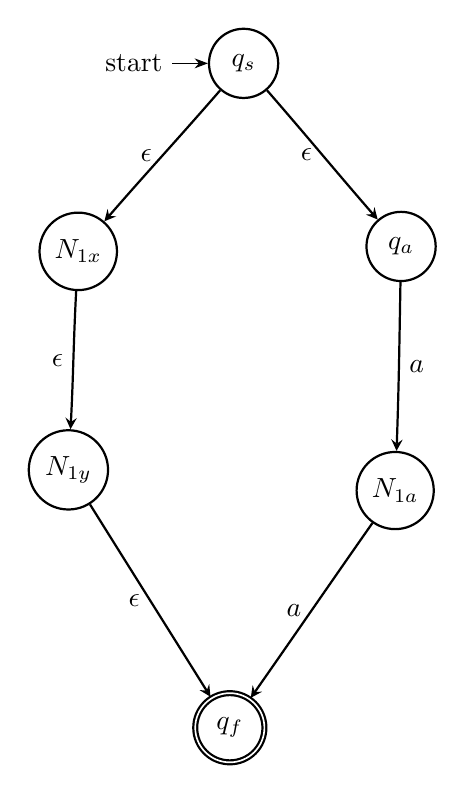
\begin{tikzpicture}[]
    \node[thick,accepting,state] at (-3.1,-4.25) (a461b17a) {$q_f$};
    \node[thick,state] at (-5.025,1.8) (b4271c25) {$N_{1x}$};
    \node[thick,state] at (-5.15,-0.975) (27837208) {$N_{1y}$};
    \node[initial,thick,state] at (-2.925,4.1875) (8b444af3) {$q_s$};
    \node[thick,state] at (-0.925,1.8625) (9c172e87) {$q_a$};
    \node[thick,state] at (-1,-1.2375) (084942d1) {$N_{1a}$};
    \path[->, thick, >=stealth]
    (b4271c25) edge [left,in = 87, out = -93] node {$\epsilon$} (27837208)
    (27837208) edge [left,in = 122, out = -58] node {$\epsilon$} (a461b17a)
    (8b444af3) edge [left,in = 49, out = -131] node {$\epsilon$} (b4271c25)
    (8b444af3) edge [left,in = 131, out = -49] node {$\epsilon$} (9c172e87)
    (9c172e87) edge [right,in = 88, out = -91] node {$a$} (084942d1)
    (084942d1) edge [left,in = 55, out = -125] node {$a$} (a461b17a)
    ;
\end{tikzpicture}
\end{center}
$N_2$ is defined as $N_2=(Q_2, \sum, \Delta_2, q_s, {q_f})$.

The NFA works, as it starts at state $q_s$, and can transition to branch $xy$, or branch $axa$ on $\epsilon$. In branch $xy$, $x\in{L(N_1)}$ is validated through $N_{1x}$. $N_2$ is able to transition to $N_{1y}$ on $\epsilon$, which validates $y\in{L(N_1)}$. Finally, $N_2$ reaches the final state $q_f$ on $\epsilon$.
In branch $axa$, $N_2$ transitions to $N_{1a}$ on $a$ in order to fulfill the condition of $axa$. $N_{1a}$ validates $x\in{L(N_1)}$. Then, $N_2$ transitions to the final state $q_f$ on $a$, completing the condition of $axa$.

\stepcounter{section}
\section*{\thesection.}

$N$ is defined as $N=(Q, \sum, \Delta, q_s, {q_f})$.

$N$ functions by starting at $q_s$. $N$ loops through $q_s$ for every $\delta\in\sum$ in order to reach $v$. $q_s$ then $\epsilon$ transitions to $M_1$ in order to validate $v\in{L(M_1)}$. After validating, $N$ $\epsilon$ transitions to $q_1$, which loops for every $\delta\in\sum$ of $w$ in order to reach $y$. $q_1$ then $\epsilon$ transitions to $M_2$ in order to validate $y\in{L(M_2)}$. After validating, $N$ $\epsilon$ transitions to the final state $q_f$. There is no need to loop through $\delta\in\sum$ for $z$, as $z\in\sum^*$ holds trivially.

\stepcounter{section}
\stepcounter{subsection}
\section*{\thesubsection}
\begin{center}
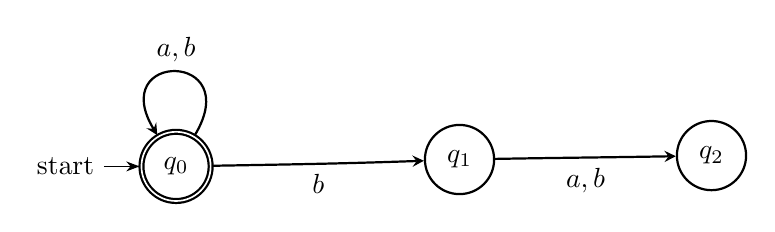
\begin{tikzpicture}[]
    \node[initial,thick,accepting,state] at (-7.275,2.8) (ab77f809) {$q_0$};
    \node[thick,state] at (-3.675,2.8875) (669cf997) {$q_{1}$};
    \node[thick,state] at (-0.475,2.9375) (ec975ff9) {$q_{2}$};
    \path[->, thick, >=stealth]
    (ab77f809) edge [loop,min distance = 1.25cm,above,in = 121, out = 59] node {$a,b$} (ab77f809)
    (ab77f809) edge [below,in = -178, out = 1] node {$b$} (669cf997)
    (669cf997) edge [below,in = -179, out = 1] node {$a,b$} (ec975ff9)
    ;
\end{tikzpicture}
\end{center}
\stepcounter{subsection}
\section*{\thesubsection}
\begin{center}
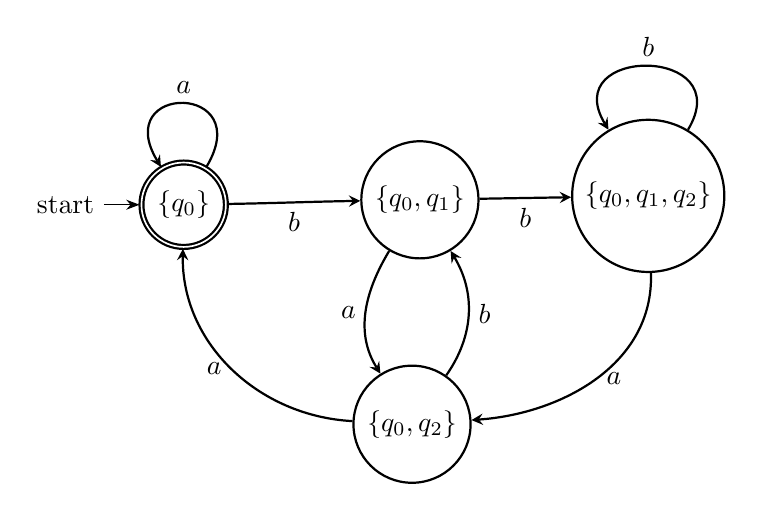
\begin{tikzpicture}[]
    \node[initial,thick,accepting,state] at (-4.5,3.25) (4f2c487a) {$\{q_0\}$};
    \node[thick,state] at (-1.5,3.3125) (880158d4) {$\{q_0,q_1\}$};
    \node[thick,state] at (-1.6,0.4625) (08d3d254) {$\{q_0,q_2\}$};
    \node[thick,state] at (1.4,3.3625) (826900e1) {$\{q_0,q_1,q_2\}$};
    \path[->, thick, >=stealth]
    (4f2c487a) edge [below,in = -179, out = 1] node {$b$} (880158d4)
    (4f2c487a) edge [loop,min distance = 1.25cm,above,in = 121, out = 59] node {$a$} (4f2c487a)
    (880158d4) edge [left,in = 122, out = -121] node {$a$} (08d3d254)
    (880158d4) edge [below,in = -179, out = 1] node {$b$} (826900e1)
    (08d3d254) edge [left,in = -91, out = 177] node {$a$} (4f2c487a)
    (08d3d254) edge [right,in = -59, out = 55] node {$b$} (880158d4)
    (826900e1) edge [right,in = 4, out = -88] node {$a$} (08d3d254)
    (826900e1) edge [loop,min distance = 1.25cm,above,in = 121, out = 59] node {$b$} (826900e1)
    ;
\end{tikzpicture}
\end{center}

\end{document}